\section{The History}
\label{sec::history}

\subsection{1996-1997: The Early Days}

January 1996, two young players that identified themselves on-line as "\textit{Spleenripper}" and "\textit{Dr. Rigormortis}" were already building new systems and preparing a full LAN set-up to get ready for the release of Quake \citep{clanHistory} \textbf{It was already a phenomenon} within its own niche before it was even a tangible game you could play and said release was still half a year hence.\\


The first relevant version of Quake that hit the public was \textit{QTest} \citep{qtest} on February 24, 1996. It became extremely popular amongst \textbf{players that already knew about \textit{Doom}} \citep{game:doom} and were eager to see the next big thing from \textit{id Software}. This version only could be played in multi-player, which shows the emphasis that the devs put on that aspect of the game.\\

Soon after that came the shareware edition of Quake. By this time the \textbf{formation of clans} such as \textit{The Amish}, \textit{Red Dragon} or \textit{Impulse 9} was already established in the community. The fact that these clans were astonishingly passionate about the game mixed with the gaming web boom at the time with some pages like \textit{Blue's News} hitting consistently 40.000 views a day. This created the perfect hotbed for the growth of such a new and fervent community.\\

Soon came the real deal, \textbf{the commercial release of \textit{Quake}} \citep{game:quake1} \textbf{in May 1996} only heated the circumstances. Talks about creating tournaments were being held every day at the forums and some started to happen, these were both small by current standards but big for the time. Also, the first QuakeCon \citep{quakecon} \parencite[p.~11]{van2013video} event was held in a hotel close to id Software's offices. It had 30 attendees in the first day and 100 by the end of the weekend once the news spread out.\\

\begin{figure}
	\begin{center}
		\fbox{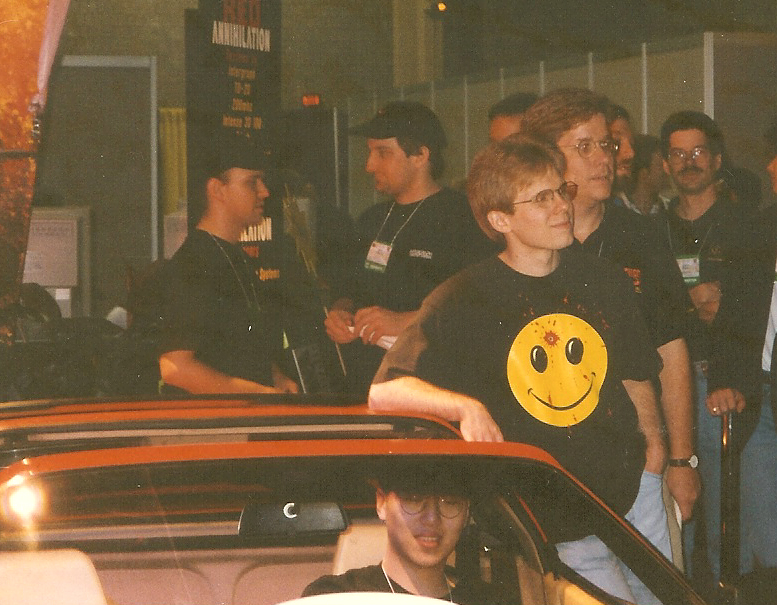
\includegraphics[width=0.95\linewidth]{resources/earlyDays.jpg}}
		
		\caption{"Thresh" wins Carmack's Ferrari. Image from \href{https://pvplive.com/c/cars-esports-prize-tournaments}{\nolinkurl{pvplive.com}}}
	\end{center}
\end{figure}

At this time nothing could compare to what happened in May of 1997 when businesses like Intergraph, Microsoft and the developers from id Software got together to organize the biggest tournament to date, they called it \textbf{\textit{Red Annihilation}s}. Said event was held during the now very famous \textbf{E3 expo} \citep{e3} in the famous \textbf{World Congress Center}.\\


This \textbf{1v1} tournament had more than 2000 participants qualifying on-line and the top 16 were flown to the live setting in the event to compete for \textbf{John D. Carmack's \footnote{John D. Carmack was the co-founder and lead developer in id Software during the era that concerns us.} Ferrari 328 GTS}. More and more breakthrough concepts kept being tied to this event. Not only the live audience was very significant but most of the spectators were able to watch the tournament via online in-game cameras professionally orchestrated. At the end of the tournament media like the NBC and The Wall Street Journal covered the event.\\

Right at that time the \textbf{CPL} \citep{web:cpl}, the pioneer in professional video-game tournament organizers, was created and a few months after, in October 1997 they organized their first event called \textbf{The FRAG} with a prize pool consisting of \$4.000 in merchandise.\\

At the end of 1997, Quake was already becoming a big hit in the gaming community and it didn't show any signs of stopping \citep{wagner2006scientific}.\\

\subsection{1998-Early 2000: Exponential growth}

\FutureContentNotesHidden{This will contain the main QuakeCon and CPL events and their growth related to the growth of eSports and the Quake community as they were.}

\textbf{\textit{Quake II}} \citep{game:quake2} was \textbf{released at the very end of 1997} and quickly became the standard for tournament play. The short intervals and significant improvements between versions of Quake had the community permanently excited to learn and compete.\\

The \textbf{year 1998} fed on the previous success and saw a significant increase in both the size of big events and the number of small ones. On July of this year, the already mentioned CPL paired with some community members involved in previous tournaments organized the third QuakeCon event, which at the same time was the second FRAG event from CPL. At the time this presented a bad view to some members of the community. Even in those circumstances, it had an attendance of 800 people and 300 BYOC \footnote{\textbf{BYOC} stands for Bring Your Own Computer, used for members of an event that carry and use their own machines.}. The prizes went from being merchandise to real money, giving \$1.000 for 5th place and scaling up to \$5.000 for first.\\

After experiencing the potential for big tournaments the \textbf{QuakeCon} dedicated more time to prepare the event without relying on the CPL. Going into the \textbf{year 1999} the event was much larger \parencite{lewis1999peace}. The major involvement from id Software as a sponsor allowed to use a much bigger venue and have developers participate. The attendance rose to 1100 people and 500 BYOC. Another important factor was the first ever tournament with \textit{Quake III} \citep{game:quake3}, which was still far from its release.\\ Later on in the year 2000, the event raised its numbers to 3000 attendees and 900 BYOC.\\

\begin{figure}
	\begin{center}
		\fbox{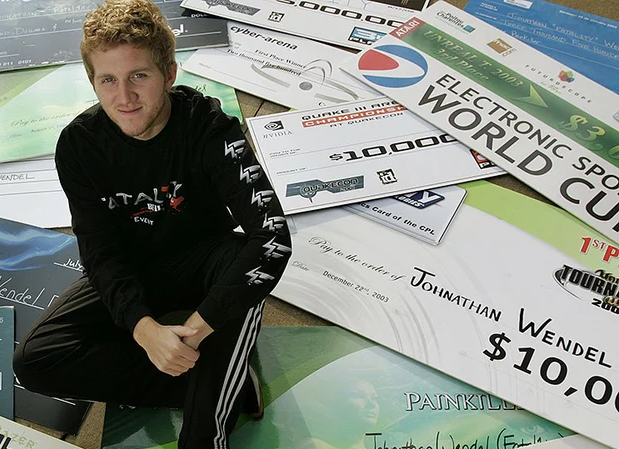
\includegraphics[width=0.95\linewidth]{resources/fatality.png}}
		
		\caption{"Fatal1ty" becoming an eSports star. Image from \href{https://www.si.com/more-sports/2016/06/30/fatal1ty-esports-professional-gaming-prize-money-motherboards}{\nolinkurl{si.com}}}
	\end{center}
\end{figure}

The \textbf{CPL} also kept blooming and establishing themselves as \textbf{the big fish in the growing pond} of eSports tournament organizers. They served as an example for many new game events and eSports leagues but none could compare to their success yet. After 1999 successful event they broke records when in the year 2000 they held a \textit{Quake III} tournament with a \textbf{prize pool of \$100.000}, 40.000 of which went to one of the rising stars of Quake, Johnathan ‘Fatal1ty’ Wendel. The existence of this characters only helped eSports and Quake to be more recognized and reach new potential fans.


\subsection{Late 2000-2001: Slayed by its own son}

\FutureContentNotesHidden{This will contain the events happened near 2001 when the main and big tournament organizers left Quake to focus on new and more liked by the public games. Mainly Counter-Strike, a game that literally came from Quake.

We can talk about how Gooseman, who worked in Quake, made the first Counter-Strike, how CS used the Quake engine as a base and how it "stole" a lot of old Quake fans and communities that naturally switches games}


\textbf{Minh "Gooseman" Le} \citep{gooseman} was a Vietnamese programmer deeply involved with the modding community of Quake. Him and another programmer in the same Quake modding team, \textbf{Jess Cliffe}, started to work on what would become the \textbf{heir of Quake} in the eSports scene, \textit{Counter-Strike} \citep{game:cs}.\\

\textit{\textbf{Counter-Strike}} came as a mod for \textit{Half-Life} \parencite{game:halflife}, the incredibly successful First-Person Shooter game based on the \textit{Quake II} engine. Le was already used to work with said engine so modding \textit{Half-Life} felt familiar. This created a very interesting situation after the first version of the mod came in June 1999.\\

CS \footnote{CS is a common abbreviation for Counter-Strike.} kept gaining fans and getting bigger by the weeks. It was the Quake's story in a much shorter time frame. Old fans from the franchise were switching to CS, tournaments quickly put it in the same position as Quake in the year 2000 and the snowball just kept fattening and rolling down an increasingly steep hill.\\

Such was its success that \textbf{2001} saw the decline of Quake by the hands of a game that was a direct successor. Quake not only gave a large part of its technology and design to CS, but also a big part of its fan-base, Quake-based tournament and league organizers and, in general, a perfect platform for the next big eSports to grow.\\

A good example was what the CPL calls the beginning of their "\textbf{Golden Years}" \citep{web:cpl}, which at the time could be considered also the golden years of eSports given the position of the organization and the creation of the World Cyber Games \citep{WCG} \parencite[p.~28]{snavely2014history}. In 2001, the event's main title was, unsurprisingly, CS replacing the long-standing Quake. This year saw a prize-pool of \$150.000 and was regarded as the biggest event to date.\\

\textbf{The leap was immense} \citep{hope2014evolution} and so the reasons to consider Quake as the main game for a tournament or league were becoming insignificant compared to the potential wins of \textbf{having CS instead}. Other new competitive games, sometimes from other growing genres, were quickly developing and feeding from the fan-bases of older games. A good example would be \textit{Starcraft} \citep{game:starcraft} representing RTSs \footnote{\textbf{RTS} is short for the Real-Time Strategy genre or games.}.\\

In general, given the deep relationship and obsession that the core of the Quake community had with the game, id Software's franchise fell to a stable and consistent position in the shadow of the biggest, more prominent games. Looking back during the beginning of the new millennium, it looked like the years of Quake ruling the early days of the eSports kingdom were long gone \parencite{edwards2013esports}.
